\documentclass[{../../master}]{subfiles}
\graphicspath{{../../}}  % 個別コンパイル時の画像パスを解決する

\begin{document}

\section{F310/F710ゲームパッドをROSで利用する}

\subsection{製品の概要}

  Logicool Gamepad F310/F710は,Logicoolから発売されているUSB接続のPC用ゲームパッドです.

  \begin{figure}[ht]
    \centering
    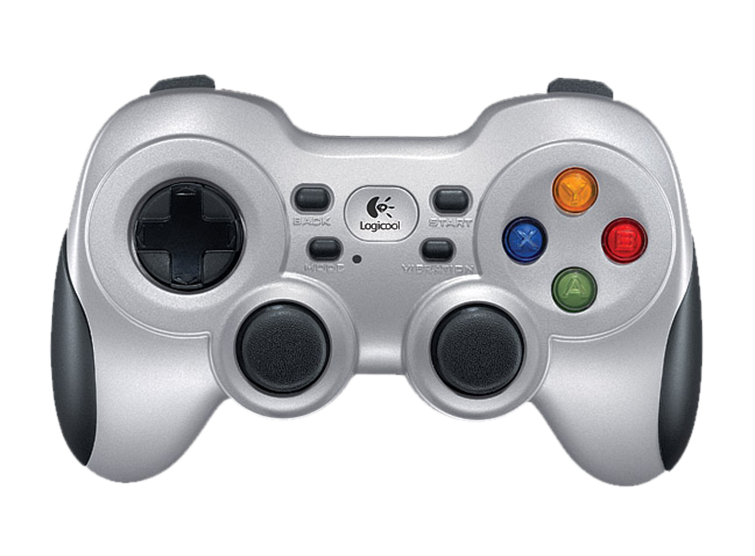
\includegraphics[width=65truemm, clip]{images/f710_overview.png}
    \label{fig:f710_overview}
    \caption{Logicool F710 Gamepad}
  \end{figure}

  有線接続のF310は2310円,無線接続のF710は4950円と安価に入手することができ,ロボットの操縦用コントローラとして使用することもできます.

\subsection{ゲームパッドの入力モード}

  310/F710ゲームパッドは2つの入力モードを持っており,物理スイッチによってモードを切り替えることができます.

  \begin{itemize}
    \item \textsf{DirectInput}モード:他のゲームパッドと同じ挙動を示すモード
    \item \textsf{XInput}モード:Xbox360コントローラをPCに繋いだときと同じ挙動を示すモード
  \end{itemize}

  \noindent
  モード切替スイッチは,F310には本体背面に,F710は本体側面上部に付いています.

  \begin{figure}[ht]
    \centering
    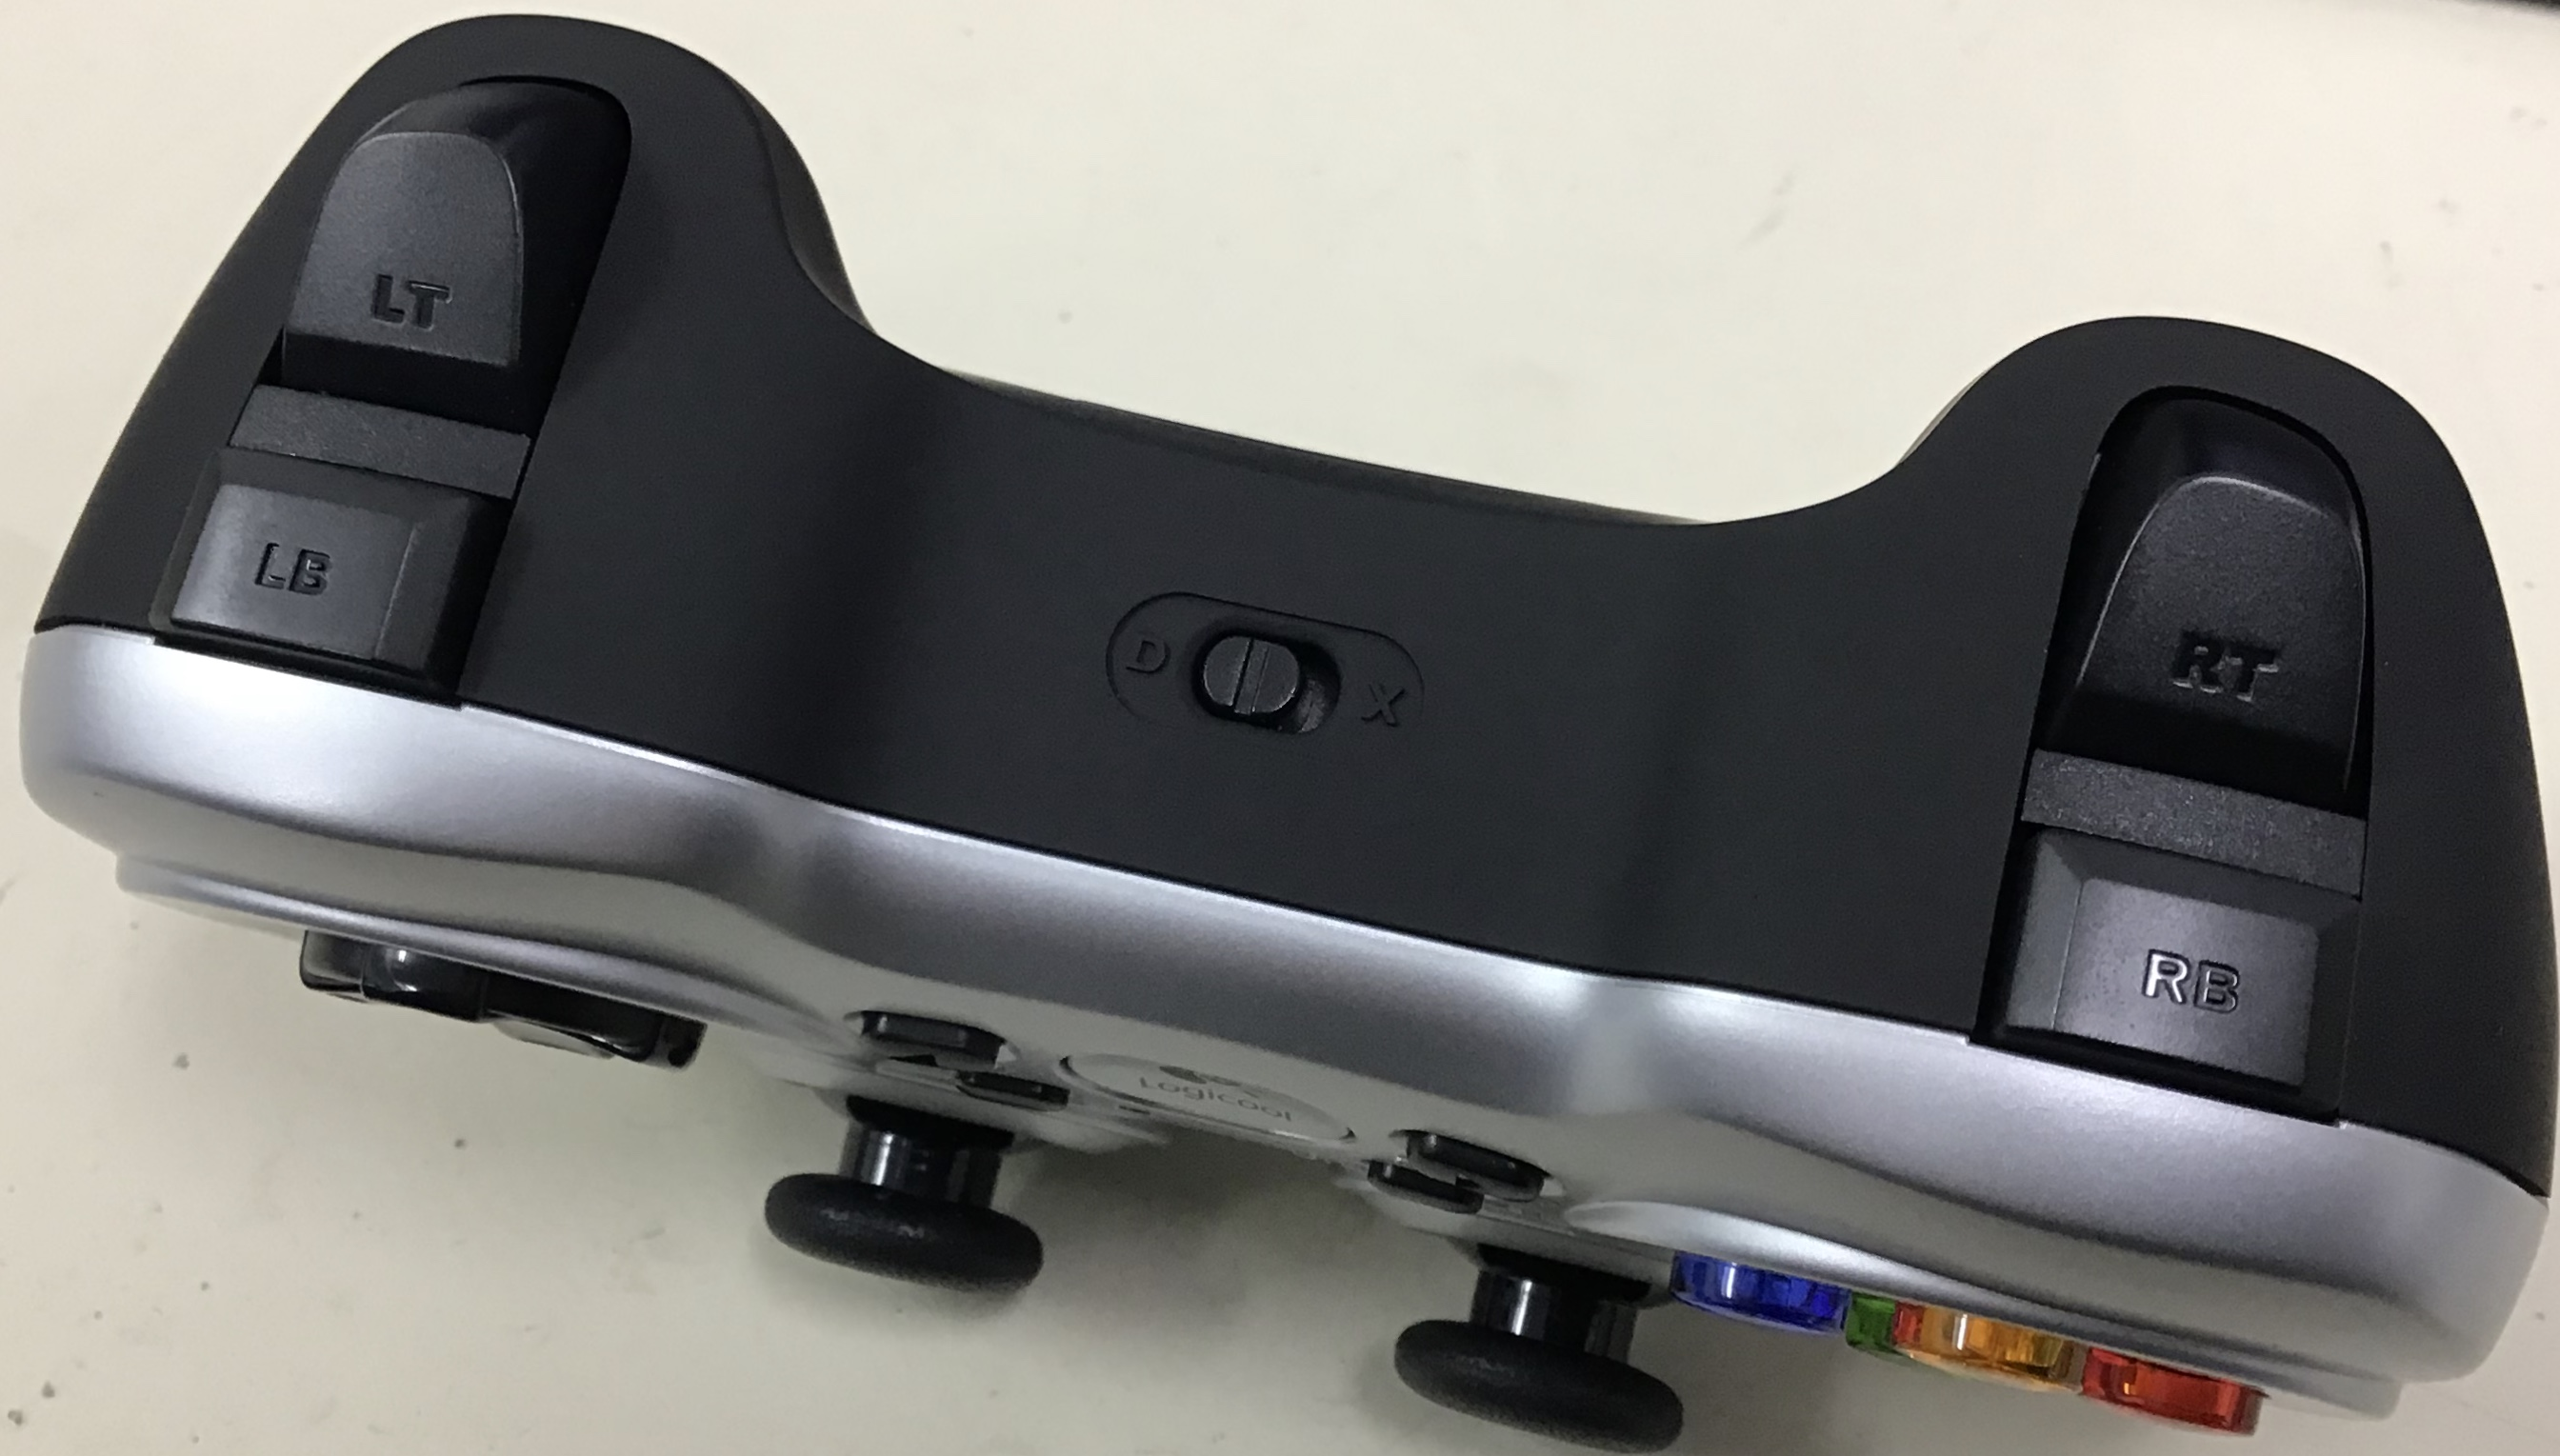
\includegraphics[clip, width=65truemm]{images/mode_switch.jpg}
    \label{fig:mode_switch}
    \caption{Mode Selector Switch for F710}
  \end{figure}

  ROSパッケージの\textsf{joy}\footnote{\url{http://wiki.ros.org/joy}}からF310/F710ゲームパッドを使用するときは,\textsf{DirectInput}モードを使用する必要があります.

\subsection{\textsf{DirectInput}モードのキーマッピング}

\textsf{DirectInput}モードでROSに接続した際のF310/F710ゲームパッドのキーマッピングを表\ref{tab:buttom_mapping}及び表\ref{tab:axis_mapping}に示します.

\textsf{sensor\_msgs/Joy}\footnote{\url{http://docs.ros.org/en/melodic/api/sensor_msgs/html/msg/Joy.html}}型メッセージでは,ゲームパッドの各軸・各ボタンの信号の値が\textsf{axes}と\textsf{buttons}の2つのリストに格納されます.
各リストに対してインデックスを指定することで,対応するボタン・軸のデータを得ることができます.

\begin{table}[h]
  \begin{center}
    \caption{Button Mapping of F310/F710 Gamepad in ROS}
    \begin{tabular}{|c|c|c|c|c|c|c|c|c|c|c|c|c|} \hline
      Buttons & X & A & B & Y & LB & RB & LT & RT & BACK & START & LeftStick & RightStick \\ \hline
       index  & 0 & 1 & 2 & 3 & 4  & 5  & 6  & 7  & 8    &   9   &   10      &     11     \\ \hline
    \end{tabular}
    \label{tab:buttom_mapping}
  \end{center}
\end{table}

\begin{table}[h]
  \begin{center}
    \caption{Axis Mapping of F310/F710 Gamepad in ROS}
    \begin{tabular}{|c|c|c|c|c|c|c|c|c|c|c|c|c|} \hline
      Axis  & Left Horiz. & Left Vert. & Right Horiz. & Right Vert. & Arrow Horiz. & Arrow Vert. \\ \hline
      index & 0 & 1 & 2 & 3 & 4  & 5 \\ \hline
    \end{tabular}
    \label{tab:axis_mapping}
  \end{center}
\end{table}

\end{document}